%% Journal version for JAIR submission — built on the official JAIR template
%% (JAIR_Example_Template.tex, September 15, 2025; acmart Revision 2.12).
%% Style commands follow the template exactly; content only.
\documentclass[manuscript, screen, review]{jair}

\setcopyright{cc}
%% \acmDOI is deliberately empty for submission: JAIR assigns the paper DOI
%% at publication, and the Zenodo deposit DOI (10.5281/zenodo.22777748) is
%% cited in the text. The JAIR class prints the bibstrip DOI label
%% unconditionally, so guard it here to suppress the line while \acmDOI is
%% empty; a non-empty \acmDOI renders unchanged.
\acmDOI{}
\makeatletter
\renewcommand{\@formatdoi}[1]{\ifx#1\@empty\else\textsc{doi:} \href{https://doi.org/#1}{#1}\fi}
\makeatother

\JAIRAE{}
\JAIRTrack{}
\acmVolume{1}
\acmArticle{1}
\acmMonth{1}
\acmYear{2026}

\RequirePackage[
  datamodel=acmdatamodel,
  style=acmauthoryear,
  backend=biber,
  giveninits=true,
  uniquename=init
  ]{biblatex}

\renewcommand*{\bibopenbracket}{(}
\renewcommand*{\bibclosebracket}{)}

\addbibresource{refs.bib}

\newcommand{\ac}[1]{\ensuremath{\alpha_c(#1)}}

\begin{document}

\title[Locality Causes Tractability?]{Locality Causes Tractability? An
Intervention Study on the Variable-Interaction Radius in Geometric Random
Satisfiability}

\author{Song Jin}
\email{j.song.cs@outlook.com}
\affiliation{%
  \institution{Independent Researcher}
  \country{China}
}

\renewcommand{\shortauthors}{Jin}

\begin{abstract}
{\bf Background:} A widespread intuition holds that real-world computational
problems are easy because their ``causes act locally'': when variables
interact only within small neighborhoods, constraint solvers should scale
well. Observational evidence supports the intuition, but observation cannot
separate locality from the many other regularities real instances carry.

{\bf Objectives:} We translate the intuition into a falsifiable, interventional
claim: holding the number of variables fixed, matching clause density relative
to each radius's own threshold, and with clause-content statistics
$r$-invariant by construction, varying \emph{only} the radius $r$ within which
clause variables are drawn from a 2-D torus should causally change
conflict-driven clause-learning (CDCL) solving difficulty.

{\bf Methods:} A locality-kernel generator sweeps nine radius levels with
preregistered threshold-matched density offsets, 30 paired seeds and two
solver engines; a degree-preserving swap chain destroys spatial locality while
keeping every literal's occurrence count exactly fixed. The protocol is
preregistered with numbered amendments, censoring semantics declared in
advance, and a prespecification-vs-implementation audit completed before
unblinding.

{\bf Results:} \emph{(i)}~The operational satisfiability boundary is not
$r$-invariant: it lies below density 2.5 at $r=0.06$ and near the classical
${\approx}4.3$ region by $r=0.22$ (a displacement of at least 1.7 density
units), before becoming unmeasurable at $r\ge 0.3$ under a
$10^7$-conflict budget. \emph{(ii)}~At density matched relative to each
radius's own threshold, difficulty spans $3.4$ orders of magnitude across $r$
among decided instances, and $\ge 4.5$ orders when budget-censored runs are
counted at their lower bound; RM-ANOVA $F(8,216)=2808.5$; Jonckheere--Terpstra
$p\le 10^{-4}$ with FDR $q\le 10^{-4}$; partial $\eta^2 \approx 0.99$.
\emph{(iii)}~The structure-destruction swap raises difficulty by
$16$--$68\times$ (Wilcoxon $p\le 7\times10^{-10}$) and flips the
satisfiability status of 53 of the 82 resolved instance pairs; the ratio
is a composite spanning those status changes (within the 29 status-stable
pairs the
elevation persists at $\times 11$ and $\times 1.8$ per offset arm,
$p\le 3.9\times10^{-3}$); post-hoc, exploratory causal
mediation analysis is consistent with ${\sim}94\%$ of the radius effect flowing
through community-structure restructuring (ACME
3.06, bootstrap CI $[2.84, 3.37]$).

{\bf Conclusions:} Locality is not merely correlated with tractability ---
under our controls it behaves as the causal channel. All claims are scoped to
$n=400$, direct CNF encodings, and CDCL-family solvers; we discuss what this
does and does not say about P versus NP. Code, seeds, data, preregistration,
and the full audit trail are public.
\end{abstract}

\maketitle

\section{Introduction}
\label{sec:intro}

\paragraph{The conjecture and its observational gap.}
In popular discussions of \textsc{P} versus \textsc{NP}, one encounters a
philosophical diagnosis: problems resist algorithmic solution when variable
interactions are strongly correlated at long range; the computational world is
tractable because causation is local. As stated, the claim is unfalsifiable
--- ``locality'', ``correlation'', and ``cause'' are unoperationalized. Yet the
intuition has an empirically serious core. Industrial SAT instances, the
reason conflict-driven clause-learning (CDCL) solvers~\cite{marques2009}
routinely decide formulas with millions of variables from competition and
application repositories~\cite{satcomp}, exhibit community structure, small
backdoors, and heavy-tailed variable-incidence patterns. Observationally,
structure and ease co-occur.

Observation, however, cannot license a causal reading. Instances that are easy
and local are also many other things. The literature's own cautionary results
make the point sharp. \citet{zulkoski2018}, in the largest
correlational study to date (${\sim}7000$ competition instances), found that
\emph{no single} structural parameter significantly predicts CDCL runtime
across heterogeneous benchmark sets. The best six-feature regression reaches
adjusted $R^2 \approx 0.31$ on application instances, and the
size-plus-treewidth feature set reaches only $0.05$. \citet{mull2016} prove that
any ``polynomial-clique'' community metric, including modularity, admits
instances with excellent scores that remain \textsc{NP}-hard, and that
pseudo-industrial community-attachment instances require exponentially long
resolution proofs with high probability when communities are few. Structure,
by itself, neither certifies nor explains tractability.

\paragraph{What an intervention adds.}
The remedy is standard in the empirical sciences and rare in SAT difficulty
research: hold everything else fixed and turn one knob. We operationalize the
locality conjecture as a dose--response experiment. A \emph{locality-kernel
generator} samples each clause's variables uniformly from an $r$-ball on a
discrete 2-D torus and draws polarities from a standardized content
distribution whose statistics are $r$-invariant by construction
($\sigma$-redundancy histograms identical across $r$ in pilots). Literal-degree
means equal $3\alpha$ exactly, varying across $r$ only through the
threshold-matched density $\alpha$, and the intervention arm's
degree-preserving swap holds the degree profile exactly fixed. The knob $r$ has a physical
reading: it is the \emph{spatial span of variable interaction} --- the exact
quantity the philosophical conjecture is about.

\paragraph{Contributions.}
\begin{enumerate}
\item \textbf{The first controlled intervention scan of locality radius.}
Nine $r$ levels $\times$ three preregistered offsets $\Delta$ above each radius's
\emph{own} operational threshold $\ac{r}$ $\times$ 30 paired seeds $\times$ two
solvers, with per-instance structural metrics (treewidth bracketed by min-fill
upper and degeneracy lower bounds; modularity, community metrics, spectral
gap). A fourth offset, $\Delta{=}{+}0.6$, is included at 4 of the 9 radii; the
$r{=}0.06$ anchors are the lattice-nearest S0 grid value 2.6 (the grid shows
the true boundary lies below 2.5), which keeps the threshold-displacement
claim a conservative lower bound and over-doses the $r{=}0.06$ scan cells by
a bounded amount, quantified in \S\ref{sec:setup}.
\item \textbf{A threshold curve $\ac{r}$} (832 solves at $10^7$-conflict
budget): the operational threshold is not $r$-invariant: the boundary lies below
2.5 at $r=0.06$ and near ${\approx}4.3$ by $r=0.22$, before difficulty
saturates beyond measurable range at $r\ge0.3$; the \emph{measurability
boundary itself} tracks $r$.
\item \textbf{A structure-destruction intervention (E3b).} A degree-preserving
swap chain destroys spatial locality while keeping the literal degree sequence
exactly fixed; paired Wilcoxon tests isolate the causal contribution of
spatial structure.
\item \textbf{Topology $\times$ content decomposition}, with the content arm's
operationalization registered openly as an amendment (AMEND-3) rather than
shipped ill-defined.
\item \textbf{An honest negative-result protocol}: preregistration frozen
before the main scan, numbered amendments, a prespecification-vs-implementation
audit that caught one material bug before unblinding, and quantitative
triggers under which we would have reported ``density dominates''.
\end{enumerate}

\paragraph{Scope.}
All claims concern CDCL-family solvers on direct CNF encodings at $n=400$ with
conflict-count difficulty. We make no claim about \textsc{P} versus
\textsc{NP} (\S\ref{sec:discussion}). Machine-independence is obtained by
using conflict counts, not wall-clock, as the primary measure.

\section{Related Work}
\label{sec:related}

\paragraph{Structural measures and CDCL performance.}
\citet{ansotegui2009} introduced the scale-free (power-law) variable-incidence
model of industrial-like instances, later extended with
fractal-dimension analyses of incidence graphs \parencite{ansotegui2014}, as
tabulated in \parencite{zulkoski2018}; \citet{newsham2014} reported encouraging
runtime regressions on
community features. \citet{zulkoski2018} scaled the design to
${\sim}7000$ instances from SAT Competitions 2007--2016 with MapleCOMSPS
runtimes and OLS/ridge regression over standardized features with full
pairwise interactions. Their findings anchor our baseline expectations:
no single parameter is significantly predictive in the aggregate; best
combos reach adjusted $R^2 \approx 0.31$ (application), $0.56$ (crafted),
$0.66$ (random); the size-plus-treewidth feature set carries almost no
explanatory power on application instances (adjusted $R^2 \approx 0.05$);
sub-category correlations are strong but \emph{sign-flipping}
(e.g.\ a mergeability ratio: Spearman $+0.94$ on argumentation, $-0.73$ on
hardware); and pre-simplification plus corpus grouping materially change
$R^2$ --- a sensitivity we inherit and control by reporting both calibers.
On the behavioral side, Zulkoski et al.\ show CDCL branching (VSIDS, LRB) is
spatially local with respect to variable-incidence-graph communities (Gini
$0.50$--$0.52$ vs $0.16$ for random branching) and temporally local (45--55\%
of decisions land in the most recent 1\% of communities). \citet{li2022}
document the hierarchical community structure of practical
instances.

\paragraph{Locality and heterogeneity: theory.}
\citet{blasius2022} prove that heterogeneity alone does not
make random $k$-SAT easy (superpolynomial resolution size), whereas geometric
locality yields small unsatisfiable subformulas findable in polynomial time ---
the strongest existing theorem-level support for ``locality $\Rightarrow$
tractability'', and the regime map our generator navigates.
Gir\'aldez-Cru and Levy's locality-based generator
variants~\cite{giraldez2017};
\citet{mull2016} then proved average-case hardness for
community-attachment instances with few communities, and showed
experimentally that \emph{community size, not formula size, dominates
runtime}: instances differing $55\times$ in variables but matched in community
size differ ${\sim}3\times$ in runtime --- an observational precursor of our
interventional question. \citet{jia2005} analyze planted
SAT via solution hiding; their planting threshold is consistent with naive planted
ensembles being CDCL-trivial, a pilot finding that motivated our non-planted
difficulty carrier.

\paragraph{Proof complexity: the width backbone.}
\citet{atserias2008} characterize resolution width
combinatorially, yielding $w(F\vdash\bot) \ge \mathrm{tw}(\text{primal}) - 2$
for 3-CNFs.
\citet{ben1999} relate width to size,
$S \ge \exp(\Omega((w-w_0)^2/n))$: a ``width barrier'' at
${\approx}\sqrt{n\log n}$. \citet{atserias2011} and
\citet{beame2003} connect CDCL to (bounded-width) resolution.
Together: low treewidth $\Rightarrow$ short proofs exist $\Rightarrow$
CDCL with restarts finds them in polynomial time --- the theoretical face of
our E1 result (\S\ref{sec:e1}: width-controlled instances are flat and
trivial at all $k$).
Correlation decay~\cite{weitz2006} and the overlap-gap property
(see \parencite{gamarnik2021}) delineate where local information provably suffices
or fails; we use these as interpretive scaffolding only, since practical CDCL
carries components outside these models.

\section{Problem Setup and Instance Generators}
\label{sec:setup}

\paragraph{Locality kernel (\texttt{geo\_random}).}
Fix $n=400$ variables placed uniformly on a discrete 2-D torus of side
$\sqrt{n}$. Each of $m=\alpha n$ clauses: pick a centre uniformly, collect the
variables within torus distance $r$ (up to 1000 attempts to find a ball
containing at least three variables), sample 3 distinct variables from that
ball, and draw polarities uniformly
(\texttt{planted=False}). Small $r$ gives high intra-cluster variable reuse
and sparse inter-cluster coupling; $r\to\infty$ recovers approximately uniform
random 3-SAT. Because the torus diameter is ${\sqrt{2}}/{2}\approx0.71$, the
$r{=}0.8$ and $r{=}1.5$ levels (whose $r$-ball spans all $n$ variables)
generate identical clause sets; sensitivity analyses treat them as one level.
A \emph{planted} variant draws polarities from
$\sigma$-satisfaction modes built on a global assignment $\sigma$: for the
$k$ positions a clause satisfies $\sigma$ on, a cardinality is drawn uniformly
in $1\ldots k$ and then a subset of that cardinality; a decoy assignment
$\beta$ instead constrains the fill of the hidden clause fraction (the
$q_{\text{hidden}}<1$ arm). Clause-content statistics are therefore
$r$-invariant by construction: redundancy histograms are identical across $r$
(verified in pilots; measured mean $\sigma$-redundancy ${\approx}2.2$).

\paragraph{Width-controlled family.}
$k$-tree skeletons give constructive treewidth $\le k$; matched random
families at the same $(n,\alpha)$ provide controls. Planted and unplanted arms
separate ``having a solution planted'' from ``being structured''. Outcomes are
reported as \S\ref{sec:e1}.

\paragraph{Structure-destruction intervention (E3b).}
A bipartite swap chain (MCMC edge swaps on the variable--clause incidence
graph, rejecting swaps that duplicate a variable in a clause or create
complementary-literal pairs) destroys spatial locality while preserving every
literal's degree \emph{exactly}. The swapped instance is not a draw from the
\texttt{geo\_random} distribution; per our preregistration we report it as a
structure-destruction intervention, and record solver-status flips per pair
explicitly.

\paragraph{Topology $\times$ content factorial.}
The topology channel is original vs.\ swapped incidence graph. The content
channel's unambiguous operationalization on our unsatisfiable-arm carrier is
non-trivial (a distribution-preserving polarity resample is the identity by
construction there); we registered this tension openly as AMEND-3 and deferred
the interaction test rather than shipping an ill-defined arm. The topology
channel is fully executed (E3b).

\paragraph{Threshold matching.}
Difficulty near threshold is U-shaped in density, so comparing arms at fixed
absolute $\alpha$ confounds $r$-effects with threshold proximity. A dedicated
threshold study (S0, \S\ref{sec:s0}) estimates the operational threshold
$\ac{r}$ per radius; the main scan samples at $\alpha = \ac{r} + \Delta$,
$\Delta \in \{+0.2, +0.4, +0.8\}$, plus a post-freeze fourth offset
$\Delta{=}{+}0.6$ at 4 of the 9 radii (deviation E3b-$\Delta$). At $r{=}0.06$ the dosing anchor is the
lattice-nearest S0 value 2.6 rather than a measured crossing (the S0 grid
there never reaches a $0.5$ SAT rate, $0.31 \to 0.13$ over densities
$2.5$--$3.1$, so the true boundary lies below the probed range); the
realized offsets therefore exceed the nominal $\Delta$. The consequence is
claim-specific: it keeps the threshold-displacement claim
(\S\ref{sec:s0}) a conservative lower bound, while for the scan comparisons
it over-doses the easy end --- difficulty at $r{=}0.06$ falls with dose
($1.45/1.40/1.29$ across the three arms; Table~\ref{tab:e3afull}) --- so the
cross-$r$ span and the gradient's steepness are mildly
\emph{anti}-conservative, on the order of $0.1$--$0.2$ decades (the
$r{=}0.06$ arm endpoints span $0.16$ decades across a $0.6$-unit dose
difference; the crossing below the probed range is undetermined).

\section{Measures, Solvers, and Statistical Protocol}
\label{sec:method}

\paragraph{Difficulty.}
Primary: $\log_{10}(\text{conflicts}+1)$ under CaDiCaL, conflict budget
$10^6$ (main scan) / $10^7$ (threshold study). CaDiCaL's budget mechanism
counts decided conflicts precisely, giving machine-independent censoring.
Secondary: wall-clock (same machine), Glucose cross-checks. A 300\,s
subprocess-isolated wall guard returns status \textsc{walltimeout} for runs
where conflicts are sparse but propagation explodes; these rows carry no
conflict count, are excluded from conflict analyses and from the
Kaplan--Meier estimation (their censored-mass trend is reported separately,
\S\ref{sec:e3a}); their directional bias is declared (AMEND-2):
truncation falls disproportionately on the \textsc{unsat} side near
threshold, which \emph{raises} resolved-SAT rates and pushes $\ac{r}$ upward
--- an anti-conservative bias for our gradient hypothesis, bounded by
spot-checks at $10^8$ conflicts / 480\,s on flagged radii
(\S\ref{sec:threats}).

\paragraph{Structural measures.}
Treewidth is reported as a bracket: min-fill upper bound (validated against
$k$-tree constructions) and degeneracy-based lower bound. Community structure
(Leiden, fixed resolution), modularity, spectral gap, redundancy histograms;
all metrics are computed deterministically on the generated instance and
stored with it.

\paragraph{Statistics.}
Repeated-measures ANOVA with seed as subject (seeds shared across all
$r\times\Delta$ cells), partial $\eta^2 = F\cdot df_1/(F\cdot df_1+df_2)$;
Jonckheere--Terpstra ordered-alternative test by Monte Carlo permutation;
paired Wilcoxon signed-rank for E3b pairs; Tobit (type-I, right-censored) and
Kaplan--Meier as censoring analyses; \citet{imai2011} causal mediation
(product-of-coefficients estimator) with bootstrap percentile ACME confidence
intervals; Benjamini--Hochberg FDR across the
primary family. Decision rules were preregistered: H2 confirmed by
FDR-corrected $p<0.05$ with partial $\eta^2 \ge 0.14$ or $\ge 10\times$
median endpoint ratio; ``density dominates'' triggered by $\eta^2<0.02$ and
$p>0.05$.

\paragraph{Preregistration and audit.}
Hypotheses, censoring semantics, $r$ levels, and decision rules were frozen
before the main scan (2026-09-09; scan completed 2026-09-10). The first
\emph{public} timestamp of the frozen documents, the amendment records
AMEND-1--4, and the audit trail is the Zenodo deposit of 2026-09-15
(\S\ref{sec:repro}); AMEND-5, dated 2026-09-18, first appeared with the
deposit's fourth version --- we disclose this freeze-to-publication gap rather than let
``preregistered'' imply an independent registry. Throughout,
\emph{unblinding} denotes the first examination of main-scan outcome
statistics; the S0 thresholds that dose the scan are examined beforehand by
design, and the audit and its one material fix predate unblinding.
Amendments are numbered and reason-stated: AMEND-1 (S0
budget $10^7$), AMEND-2 (wall guard, bias declaration, spot-check protocol),
AMEND-3 (content-arm deferral), AMEND-4 (terminology normalization and
content-arm disposition record), AMEND-5 (mediation-path adaptation with the
width-path quantification). A prespecification-vs-implementation audit
records every deviation found by item-by-item inspection --- including one
material bug (walltimeout rows initially counted as \textsc{unsat} in
threshold estimation) fixed \emph{before} the main scan fired, and the
post-freeze fourth dosing offset $\Delta{=}{+}0.6$ at 4 of the 9 radii
(deviation E3b-$\Delta$). One exploratory
arm (E6: LLM-proposed branching orderings as a candidate content channel) was
cut at its preregistered stop-line after showing no $r$-gradient signal
relative to its baseline; the cut is documented in the frozen preregistration
and the arm is recorded as a negative result. Appendix~\ref{app:protocol}
summarizes the frozen protocol, decision rules, and amendments in full.

\section{Results I: The Threshold Curve \texorpdfstring{$\ac{r}$}{alpha\_c(r)} (S0)}
\label{sec:s0}

S0 resolves 832 runs (720 preregistered grid jobs + 112 grid-floor extension
jobs) at $10^7$-conflict budget, 16 seeds per cell. With only resolved runs
contributing to SAT rates (AMEND-2 caliber) and linear interpolation of the
$0.5$-crossing (Fig.~\ref{fig:alphac}):

\begin{table}[h]
\centering
\caption{Operational threshold vs.\ locality radius. $^{*}$measurement-saturated
radii: the crossing is unidentifiable; the table carries the pilot coarse
value, flagged low-confidence, with spot-checks per AMEND-2. $^{\dagger}$the
SAT rate never reaches 0.5 on the explored grid ($\alpha\in[2.5,3.1]$, rate
${\sim}0.31$ at the grid floor declining to ${\sim}0.13$): the boundary at
$r=0.06$ is bracketed from above, not pinpointed. The complete per-cell grid
(52 cells $\times$ 16 seeds) is given in Appendix~\ref{app:s0grid}.}
\begin{tabular}{lccccccccc}
\toprule
$r$ & 0.06 & 0.08 & 0.11 & 0.15 & 0.22 & 0.3 & 0.5 & 0.8 & 1.5\\
\midrule
$\ac{r}$ & $<2.5^{\dagger}$ & 3.35 & 3.82 & 4.20 & 4.23 & 4.40$^{*}$ & 4.70$^{*}$ & 4.60$^{*}$ & 4.60$^{*}$\\
censoring & 2.1\% & 0\% & 0\% & 0\% & 0\% & 92.5\% & 98.8\% & 100\% & 100\%\\
\bottomrule
\end{tabular}

\label{tab:alphac}
\end{table}

\begin{figure}[t]
\centering
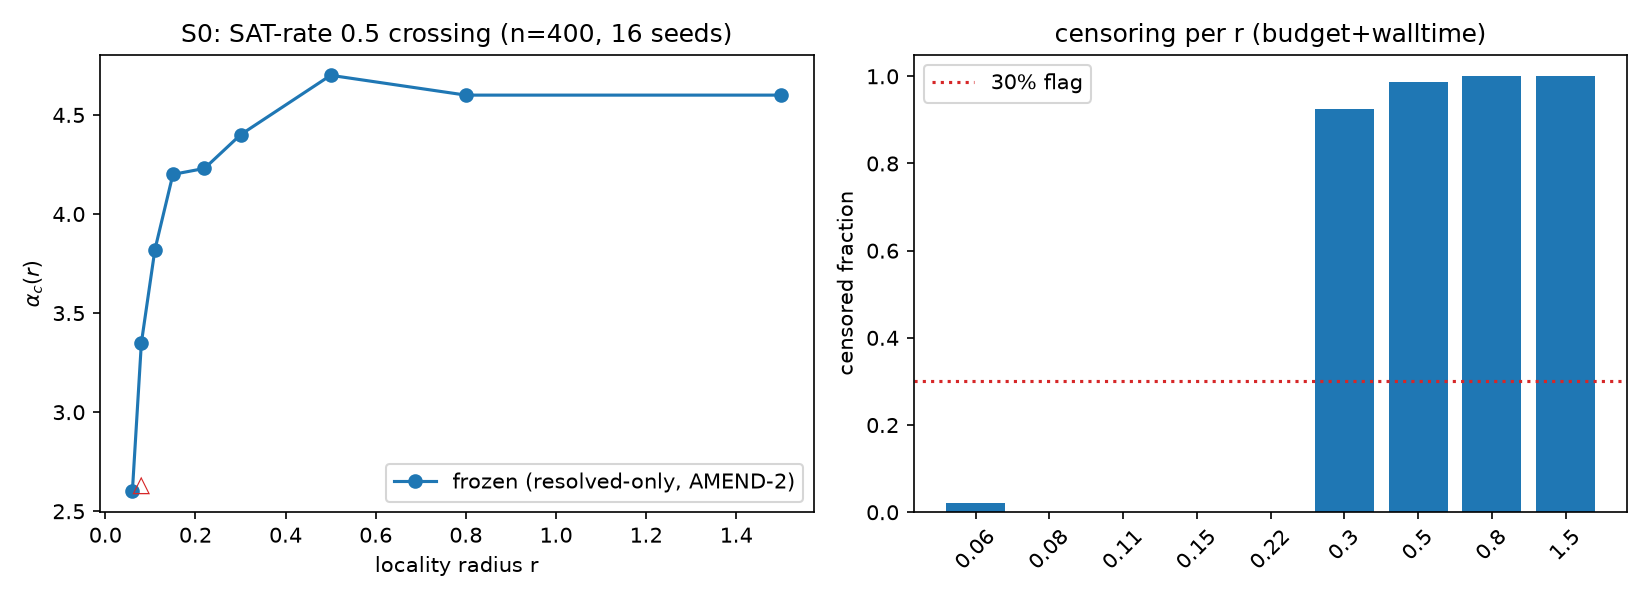
\includegraphics[width=0.85\linewidth]{figures/fig_s0_alphac.png}
\caption{Left: the operational threshold $\ac{r}$, resolved-only caliber
(AMEND-2; $\triangle$ marks radii whose grid has no $0.5$-crossing, carried at
their lattice-nearest pilot values). Right: censoring fraction per radius
(budget + walltime) --- the measurability boundary itself tracks $r$.}
\Description{Line plot of the operational satisfiability threshold as a
function of the locality radius (left panel): the threshold starts below
density 2.5 at radius 0.06, rises steeply through radius 0.22, and saturates
near 4.4 to 4.7 at large radii; triangle markers flag radii whose threshold
could not be pinpointed because the grid has no 0.5-crossing. The right panel
shows the censoring fraction per radius as bars, rising from about 2 percent
at radius 0.06 to 100 percent at radius 0.8 and above.}
\label{fig:alphac}
\end{figure}

Three observations. \emph{(i)}~The operational threshold is not
$r$-invariant. At $r=0.06$ the SAT rate is already only ${\sim}0.31$ at
density 2.5 and declines gently through 3.1 (censoring $\le2.1\%$): the
boundary is bracketed below density 2.5. By $r=0.22$ it has risen past 4.2
--- a displacement of \emph{at least} 1.7 density units. Locality does not
merely re-scale difficulty around a fixed threshold, it \emph{moves the
threshold itself}. \emph{(ii)}~The curve saturates near the classical
random-3-SAT threshold region \parencite{mezard2002} ($\alpha_c \to 4.267$ as $n\to\infty$),
consistent with $r\to\infty$ recovering uniform random 3-SAT and with the
width-backbone picture: small radii admit satisfiability far below it (the
geometric small-subformula regime of \parencite{blasius2022}). \emph{(iii)}~At $r\ge0.3$,
near-threshold instances collapse out of measurable range (313 walltimeouts
concentrated there): the question ``where is the threshold'' stops being
answerable at fixed budget --- a difficulty-regime change, bounded by
spot-checks (\S\ref{sec:threats}).

\section{Results II: Dose--Response at Matched Threshold Offset (E3a)}
\label{sec:e3a}

The main scan places 9 radii $\times$ 3 offsets above each radius's own
$\ac{r}$, 30 paired seeds, two solvers: 1740 runs, of which 1350 resolved
and 390 censored (Table~\ref{tab:e3afull}). The store additionally carries
the 240 swap-arm rows of \S\ref{sec:e3b} (86 resolved, 154 censored), for
1980 runs with zero errored rows and 544 censored overall (27.5\%,
concentrated at $r\ge0.3$); of those 544, 535 hit the $10^6$-conflict
budget and 9 the $300$\,s wall guard, which excludes at scale only in S0
(317 rows, 313 at $r\ge0.3$). Figure~\ref{fig:dose}
visualizes both arms.

\paragraph{Primary tests (CaDiCaL, $\Delta$-pooled, seeds as subjects).}
RM-ANOVA on the $\Delta$-aggregated complete-seed subset ($\Delta\in\{0.2,
0.4,0.6,0.8\}$, the $0.6$ arm present at 4 of the 9 radii; $n=28$ seeds
observed at all radii): $F(8,216)=2808.5$, $p\approx1.1\times10^{-213}$.
\emph{Scoring convention:} cell means average \emph{decided} rows only
(budget-censored and walltimeout runs are excluded, per the declared
semantics), computed per (seed, radius) across the $\Delta$ arms present, so
at heavily censored radii the mean rests on whichever arms resolved
(unequal arm weights); a seed enters the subset only if every radius
contributes at least one decided run ($28$ of $30$ seeds qualify).
Dropping the duplicate $r{=}1.5$ level (identical clause sets to $r{=}0.8$,
\S\ref{sec:setup}) gives the same conclusion,
$F(7,189)=2468.7$. Jonckheere--Terpstra (Monte Carlo permutation, $10^4$
draws): $p\le10^{-4}$
--- the resolution floor of the permutation distribution --- for every
$(\Delta, \text{solver})$ cell; BH-FDR $q \le 10^{-4}$ across the seven-member
primary family. A censoring-robust variant (censored runs scored at the
budget value) reproduces $p\le10^{-4}$, so the trend is not an artifact of
dropping censored rows. Kaplan--Meier curves of time-to-decision
(Fig.~\ref{fig:km}) make the same point visually: the median conflict count at
decision rises from 23 ($r=0.06$; identical under the Kaplan--Meier
estimator) through 20{,}695 ($r=0.22$, Kaplan--Meier median) to censoring
plateaus --- half or more undecided at $r\ge0.5$, about a quarter at $r=0.3$.

\begin{table}[h]
\centering
\caption{Dose--response at $\Delta=+0.2$ (the near-threshold arm, CaDiCaL).
$^{*}$means over surviving (easier) instances only; the censoring-aware
Jonckheere--Terpstra bounds the underlying trend. The complete per-radius
grid for all seven $(\Delta, \text{solver})$ arms is given in
Appendix~\ref{app:e3atable}.}
\begin{tabular}{lccccccc}
\toprule
$r$ & 0.06 & 0.08 & 0.11 & 0.15 & 0.22 & 0.3 & 0.5\\
\midrule
mean $\log_{10}$ conflicts & 1.45 & 1.68 & 2.30 & 3.02 & 4.86 & 5.87$^{*}$ & 5.93$^{*}$\\
resolved $n$ & 30 & 30 & 30 & 30 & 30 & 9/30 & 2/30\\
\bottomrule
\end{tabular}

\label{tab:dose}
\end{table}

\begin{figure}[t]
\centering
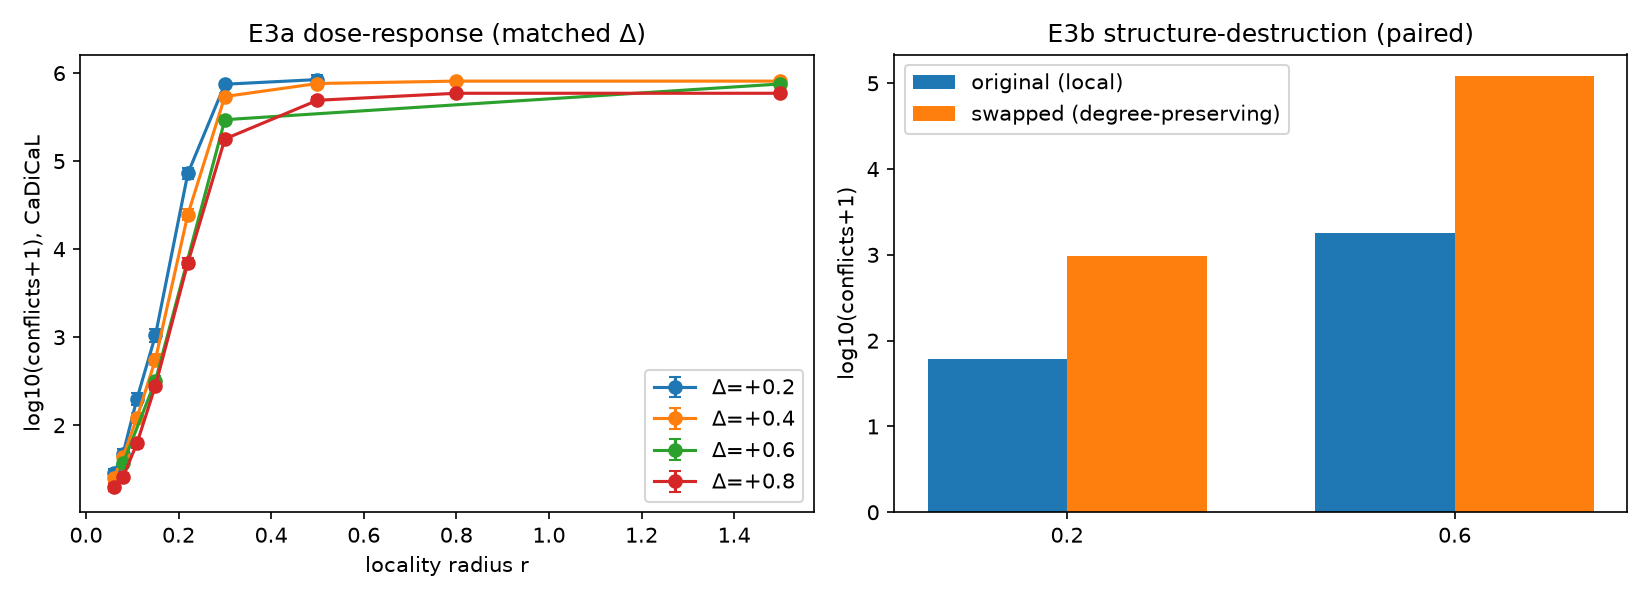
\includegraphics[width=0.95\linewidth]{figures/fig_e3a_dose.png}
\caption{Left: dose--response of difficulty to the locality radius at matched
threshold offsets (mean $\pm$ s.e.m., CaDiCaL; $\Delta{=}{+}0.8$ endpoints
$1.29$ at $r{=}0.06$ and $5.77$ at $r{=}0.8$). Right: paired
structure-destruction effect (E3b).}
\Description{Left panel: a line plot of mean log10 conflicts against the
locality radius at matched threshold offsets, rising steeply and monotonically
from about 1.3 log units at radius 0.06 to about 5.8 at radius 0.8, with
error bars. Right panel: a paired bar comparison showing that
structure-destroyed (swapped) instances are markedly harder than their
original counterparts.}
\label{fig:dose}
\end{figure}

From $r=0.06$ to $r=0.22$ at the \emph{same} threshold offset, difficulty
climbs from ${\sim}28$ to ${\sim}72{,}000$ conflicts --- \textbf{3.4 orders of
magnitude} among decided instances, and $\ge 4.5$ orders when the censored
runs at $r\ge0.3$ are counted at their budget lower bound. The
$\Delta=+0.8$ arm repeats and extends the pattern ($1.29$ at $r{=}0.06$ $\to$
$5.77$ at $r{=}0.8$,
${\approx}4.5$ orders).
Partial $\eta^2$ at computable cells is $0.985$--$0.988$ against the
preregistered confirmation threshold of $0.14$, and the $\Delta=+0.8$ arm's
endpoint ratio ${\sim}10^{4.5}$ dwarfs the preregistered $10\times$ line. \textbf{H2 is
confirmed under its own preregistered decision rule} (the statistical
branch; the degree-\emph{shape} premise holds in dispersion but not in the
max-degree tail, ${\sim}29\%$ against the frozen ${<}5\%$ criterion ---
\S\ref{sec:threats} quantifies the deviation and why the attribution does
not rest on it). Glucose replicates the
pattern.

\paragraph{$\Delta$ semantics under $\ac{r}$ bias.}
For flagged radii the $\alpha_c$ carries a bounded (and for $r\ge0.5$,
unbounded) overestimate (\S\ref{sec:threats}); this shifts the precise
horizontal placement of those cells but leaves the matched-comparison
structure (within-$r$ across $\Delta$, within-$\Delta$ across $r$)
intact, which is where the gradient evidence lives.

\begin{figure}[t]
\centering
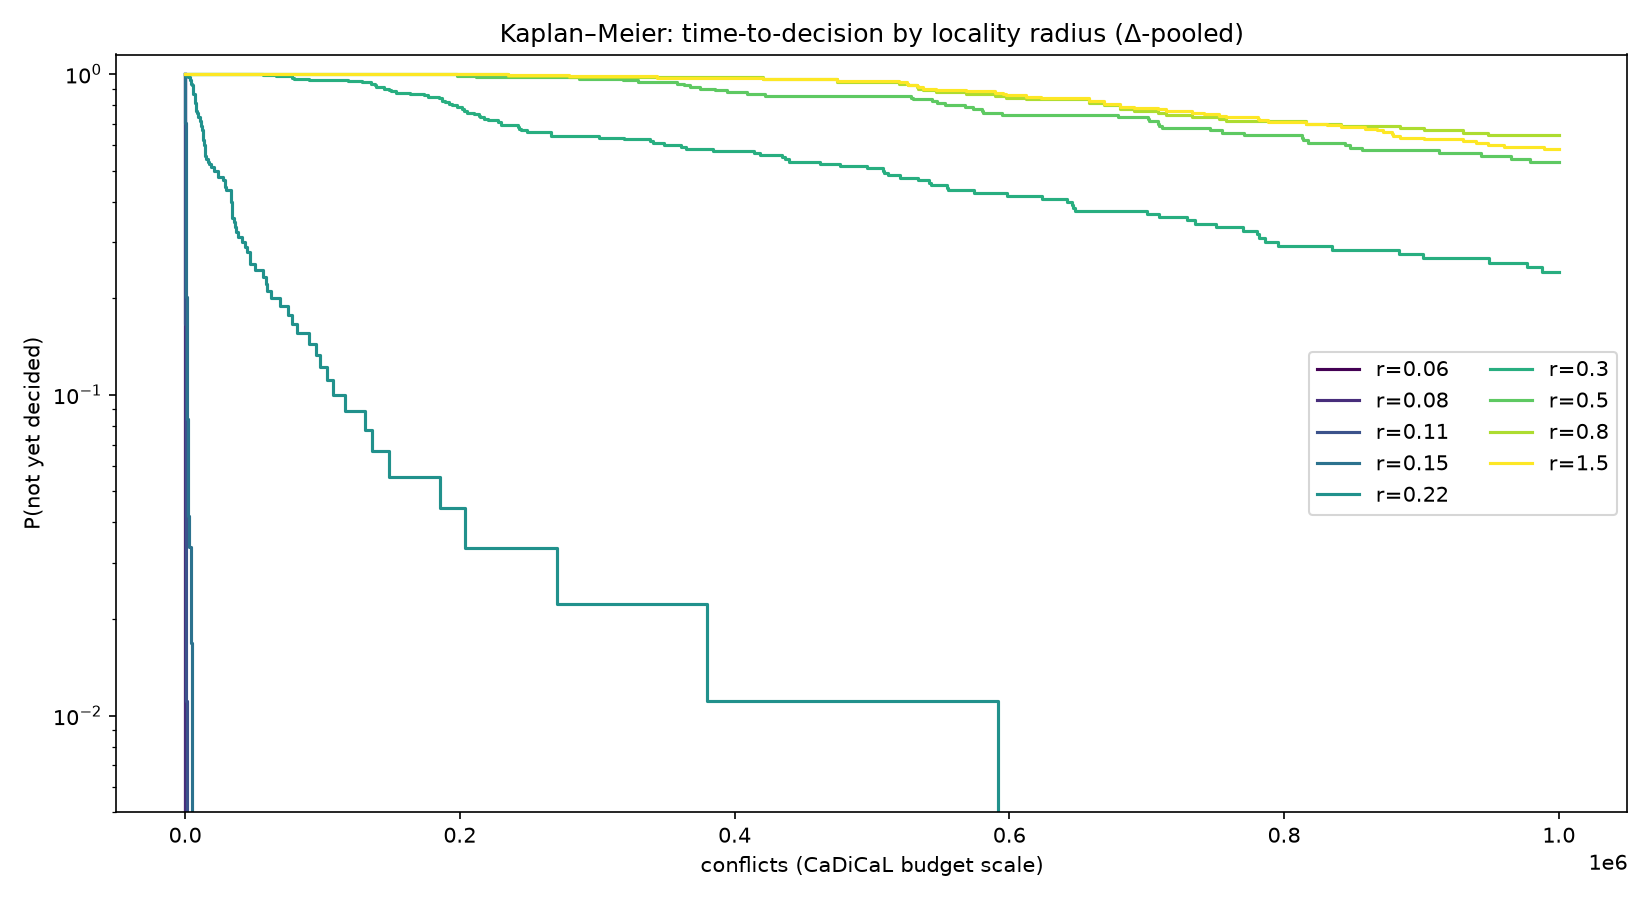
\includegraphics[width=0.9\linewidth]{figures/fig_km.png}
\caption{Kaplan--Meier estimates of time-to-decision (conflicts; CaDiCaL,
$\Delta$-pooled). Inclusion per \S\ref{sec:method}: budget-capped runs
enter as censored at the $10^6$-conflict budget; \textsc{walltimeout} rows
are excluded. Curves for small $r$ drop to zero within the budget; curves
for $r\ge0.5$ plateau at high ``not yet decided'' probability (about a
quarter at $r=0.3$) --- the
measurability boundary of \S\ref{sec:s0}, seen at the solver level.}
\Description{Kaplan-Meier curves of time-to-decision measured in conflicts
for several locality radii. Curves for small radii drop to zero well within
the budget, while curves for radius 0.3 and above plateau at high undecided
probability, about a quarter at radius 0.3 and half or more at radius 0.5
and beyond.}
\label{fig:km}
\end{figure}

\section{Results III: The Structure-Destruction Intervention (E3b)}
\label{sec:e3b}

Degree-preserving swapping holds every literal's occurrence count \emph{exactly}
fixed while destroying spatial locality. Paired Wilcoxon signed-rank:

\begin{table}[h]
\centering
\caption{E3b paired results. 53 of the 82 resolved pairs flip satisfiability
status under the swap (24 of 33 pairs at $\Delta{=}{+}0.2$; 29 of 49 at
$\Delta{=}{+}0.6$).}
\begin{tabular}{lccccc}
\toprule
$\Delta$ & pairs & original mean logc & swapped mean logc & ratio & $p$\\
\midrule
$+0.2$ & 33 & 1.79 & 2.99 & $\times 16$ & $7.0\times10^{-10}$\\
$+0.6$ & 49 & 3.25 & 5.08 & $\times 68$ & $6.0\times10^{-13}$\\
\bottomrule
\end{tabular}

\label{tab:e3b}
\end{table}

As a sensitivity check, the effect is not an artifact of comparing across
decision boundaries: within the 29 status-stable pairs (9 sat--sat at
$\Delta{=}{+}0.2$, 20 unsat--unsat at $\Delta{=}{+}0.6$), swapped instances
still take more conflicts in 25 of 29 ($\times 11$, $p=3.9\times10^{-3}$ at
$+0.2$; $\times 1.8$, $p=3.2\times10^{-4}$ at $+0.6$; pooled
$p=6.3\times10^{-7}$), with magnitudes below the pooled ratios of
Table~\ref{tab:e3b} because the flip stratum concentrates the extreme cases.
Each arm attempts 120 swap pairings (4 radii $\times$ 30 seeds;
original-arm counterparts come from the main-scan store); completions fall
to 33 and 49 because the large-radius cells saturate the budget in either
arm (at $+0.2$ the original arm decides $9/30$ and $0/30$ at $r{=}0.3$ and
$r{=}1.5$, the swap arm $0/30$ at both and $3/30$ at $r{=}0.15$).

Together with E1 (\S\ref{sec:e1}), whose width-controlled instances stay flat
and trivial at every treewidth cap, the asymmetry is sharp: what CDCL
difficulty responds to is \emph{local geometry}, not any global topological
summary.

\section{Results IV: The Width-Controlled Control Family (E1)}
\label{sec:e1}

E1 asks the complementary question to the intervention scan: if
``structure'' in the coarse topological sense were what CDCL difficulty
feeds on, then instances built to have small treewidth, the canonical
structural advantage, should be easy, and difficulty should track the
cap $k$. The $k$-tree construction gives constructive treewidth $\le k$ at
every level $k \in \{3,5,8,12,16,20\}$, at $n \in \{300,600\}$ and matched
density $\alpha = 4.0$, in two arms: a \emph{planted} arm (a satisfying
assignment built into the instance) and an \emph{unplanted} arm. Matched
random 3-SAT provides the density control (E2).

Table~\ref{tab:e1} summarizes the outcome: flat and trivial. The unplanted
arm is uniformly \textsc{unsat} at this density and refuted within at most 20 conflicts (typically single
digits), with per-$k$ medians (pooling both
sizes) confined to $7$--$10$ across the entire $k$ range (no trend in
$k$), while \emph{every} resolved planted instance (238 of them) is
decided at zero conflicts. The density control at the same $\alpha = 4.0$
(random 3-SAT, $n{=}400$, between the two widths' sizes) sits over three
orders of magnitude higher, median $21{,}011$ conflicts, exactly where
classical random-3-SAT behavior puts it. Low treewidth therefore delivers
what the width backbone predicts (\S\ref{sec:related}: short proofs exist
and CDCL finds them), and the contrast with the locality scan is the point:
at a density where width-bounded families never leave the tens of
conflicts, the geometric family spans $10^{1.45}$--$10^{4.86}$ at its
\emph{lowest} matched offset (\S\ref{sec:e3a}). What difficulty responds to
is local geometry, not any global topological summary --- and planting a
solution, the classical tractability crutch, trivializes the width-bounded
family completely.

\begin{table}[h]
\centering
\caption{E1/E2: median conflicts to decision (CaDiCaL, $10^6$-conflict
budget, $\alpha = 4.0$). Unplanted arm pools $n \in \{300,600\}$ (39--40
resolved seeds per $k$); planted arm: all 238 resolved runs decided at
zero conflicts. The density control (random 3-SAT, $n{=}400$, E2) is shown
for reference.}
\label{tab:e1}
\begin{tabular}{lcccccc}
\toprule
$k$ & 3 & 5 & 8 & 12 & 16 & 20\\
\midrule
unplanted median & 7 & 7 & 8 & 10 & 9 & 10\\
planted median & 0 & 0 & 0 & 0 & 0 & 0\\
\bottomrule
\end{tabular}
\end{table}

\section{Results V: Mediation and the Feature Ladder (H1)}
\label{sec:mediation}

\citet{imai2011} causal mediation of the $r \to$ difficulty path (bootstrap
95\% CI; total effect 3.26 log units) is summarized in
Table~\ref{tab:mediation}. The frozen protocol named treewidth as the
mediator; Appendix~\ref{app:protocol} (AMEND-5) records the adaptation of
the mediator set and quantifies the width path through the recorded
treewidth bounds (both CIs exclude zero). Because the adaptation postdates
the outcome data (AMEND-5, at independent-review disposition), we read the
whole mediation block as \emph{exploratory, supportive} mechanism evidence,
not a confirmatory test.

\begin{table}[h]
\centering
\caption{Causal mediation of the radius $\to$ difficulty path (total effect
$3.26$ log units; product-of-coefficients estimator, bootstrap percentile
CIs). Modularity carries ${\sim}94\%$ of the total effect; the spectral gap
enters as a suppressor (negative direct effect, ACME exceeding the total
effect) --- consistent with a secondary pathway, though marginal
single-mediator fits can also produce this pattern under misspecification,
so no claim rests on it. All CIs exclude zero; by the adapted rule
(Appendix~\ref{app:protocol}, AMEND-5) the block passes its criterion and is
read as exploratory, supportive mechanism evidence.}
\begin{tabular}{lccc}
\toprule
mediator & ACME & 95\% CI & direct effect\\
\midrule
modularity & 3.06 & $[2.84, 3.37]$ & $0.20$\\
spectral gap & 3.92 & $[3.68, 4.28]$ & $-0.66$\\
mean degree & 2.34 & $[2.15, 2.60]$ & $0.92$\\
clustering & 2.19 & $[2.02, 2.44]$ & $1.06$\\
\bottomrule
\end{tabular}

\label{tab:mediation}
\end{table}

The four mediators are estimated marginally (one two-step path each); several
share the same instance graphs, so the shares are not additive across
mediators.

The H1 feature ladder: on the main-scan data, ridge-CV $R^2$ rises from
$0.610$ (size features) and $0.664$ (size+density) to $\mathbf{0.976}$ with
structural features: on controlled families, structure carries predictive
power that observation on random families cannot see (random-family baseline, the E2 control of \S\ref{sec:e1}:
$0.90$ with zero structural gain). The preregistered nested OLS
$F$-test on the same subset confirms the ladder: $F(60,1283)=297.8$,
$p<10^{-4}$ for the structural block beyond size+density. A
gradient-boosted predictor with leave-one-$r$-out extrapolation (training
never sees the target radius) reaches $R^2 = 0.76$: structural features
generalize to unseen locality levels.

\section{Results VI: Placement on Real Instances (E4-prime)}
\label{sec:e4}

All 59 fetched real instances (42 combinatorial/crafted from a public
benchmark suite; 17 DIMACS classics) were solved under the S0 budget protocol:
22/59 decided. The DIMACS classics anchor the easy end: 15 \textsc{sat} and 2
\textsc{unsat}, all decided within milliseconds (an audit caught a parsing
artifact in the 1996 legacy DIMACS dialect, silently truncating these files;
they were re-solved after the fix, with the full trail in the repository log).
The combinatorial challenge instances mostly exceed the wall guard (hard
anchor); file-name labels match our determinations on every checkable Heule
instance, though one legacy \texttt{-yes} file is in fact \textsc{unsat}. Our
generator's difficulty spectrum spans the middle of the real spectrum from
textbook-easy to competition-hard. The industrial-diversity caveat stands
(\S\ref{sec:threats}).

\section{Threats to Validity}
\label{sec:threats}

\paragraph{Construct.}
``Locality radius $r$'' is one spatial operationalization on a 2-D torus host;
other hosts and other notions may disagree. Our claim is about $r$ as defined.
Difficulty is conflict counts under CDCL --- a proxy for, not a definition of,
hardness.

\paragraph{Internal.}
Five controls close the confounding routes we identified: the variable count
$n$; the density $\alpha$ (fixed or $\Delta$-matched); the literal degree
profile (degree-cap rejection in the planted arms; \emph{exact} preservation
under the E3b swap, the decisive control); the clause content (standardized
polarity sampling, $r$-invariant redundancy); and the solver engine (two
engines, both VSIDS-family CDCL; the registered local-search prediction of
\S\ref{sec:discussion} is the declared probe beyond that family). Metrics are computed deterministically before solving, so the
metric-computation channel cannot pseudo-correlate with runtime. Censoring is
the residual internal threat: the wall guard is directionally biased
(AMEND-2), and the direction was declared before unblinding. Spot-checks at
$10^8$ conflicts bound the $\alpha_c$ bias. At $r=0.3$, \textsc{sat}
instances appear $0.2$ below the operational threshold (bias $\in[-0.2,0]$
density units); at $r\ge0.5$, the $\pm0.2$ offsets fail to bracket the
boundary at $10^8/480$\,s, since every instance at $\alpha_c+0.2$ is decided
\textsc{unsat} while those at $\alpha_c-0.2$ stay undecided. The
measurability boundary is thus robust, and the flagged $\alpha_c$ values
carry an unbounded-bias caveat.
One material implementation
deviation was caught by the prespecification audit \emph{before} unblinding
and fixed; the trail is public.

\paragraph{Literal-degree profile.}
Because density is $\Delta$-matched to each radius's own threshold, the mean
literal degree ($3\alpha$: $8.4$ at $r=0.06$ vs.\ $14.7$ at $r=0.5$ in the
$\Delta{=}{+}0.2$ arms) necessarily co-varies with $r$; this is inherent to
threshold matching, and standardized by measuring density as a distance from
each radius's own boundary. The \emph{shape} of the literal-degree
distribution, however, is monitored rather than enforced in the main
\texttt{geo\_random} family. Across the $\Delta{=}{+}0.2$ cells (30 seeds
each) the per-cell worst-case maximum degree spans $24$--$31$ across $r$
(${\sim}29\%$ above the low-$r$ endpoint), exceeding the ${<}5\%$ matching
criterion laid down in the frozen H2 premise; the per-cell standard
deviation stays within it ($3.75 \to 3.85$, ${\sim}3\%$). We disclose this
deviation rather than silently incur it. It does not carry the causal
attribution, which rests on the E3b swap alone: that intervention preserves
the literal occurrence counts of every instance \emph{exactly}, so the
$16$--$68\times$ paired difficulty shift cannot be carried by degrees. We do
not lean on the direction of the residual shape drift, because the two tail
readings point opposite ways: absolute tails grow toward the \emph{large}-$r$
end (where heavier tails are typically the \emph{easier} regime for CDCL),
while the relative dispersion falls (coefficient of variation ${\sim}0.45 \to
0.26$ across $r$), i.e.\ the small-$r$ end is the relatively heavier-tailed
one. Either reading leaves the causal claim unchanged. A degree-capped
\texttt{geo\_random} variant remains an open robustness arm.

\paragraph{External.}
\texttt{geo\_random} is an intervention vehicle, not a survey of practice;
the real-instance placement is restricted to decided instances, with the
industrial-diversity caveat documented (the canonical SAT 2024 main-track
files were unreachable from our network; the deterministic preselection table
(400 instances with hashes and 15-solver reference runtimes) is retained
in the authors' working archive for future completion). All conclusions are scoped to CDCL-family solvers, direct CNF
encodings, $n=400$, and conflict-count difficulty.

\paragraph{Statistical conclusion.}
Paired designs with 30 seeds per cell, preregistered effect-size thresholds,
FDR over the primary family, and censoring-robust cross-checks. No formal
power analysis was performed for the negative branch: 30 seeds per cell
was set by the compute budget at design time, and the prespecification
audit's design-stage power note (a minimum detectable paired effect of
$dz\ge0.52$ at power $0.80$ under pilot dispersion, i.e.,
${\sim}0.2$--$0.3$ orders of magnitude between adjacent cells) does not
extend to a power calculation under the realized censoring --- the
negative-branch trigger ($\eta^2<0.02$ with $p>0.05$) therefore carries
none, the confirmatory branch is insensitive to this (observed effects
exceed the thresholds by orders of magnitude), but the negative branch's
interpretability would have rested on it.

\section{Discussion: What This Does and Does Not Say About P vs NP}
\label{sec:discussion}

Nothing we measure bears on \textsc{P} versus \textsc{NP}. The conjecture we
test descends from a philosophical \emph{intuition} about why the
computational world feels tractable --- ``causes act locally'' --- and
intuitions of this kind deserve attention precisely because they can be
operationalized and then shot down.

\paragraph{Phase transitions and a portable diagnostic.}
A classical observation, dating to Cheeseman, Kanefsky and Taylor's
``Where the really hard problems are''~\cite{cheeseman1991}, holds that
combinatorial problems are hardest near structural phase transitions. Our
results give that observation a \emph{causal, solver-relative} reading for
SAT/CDCL: the locality radius moves the transition itself and restructures
difficulty within matched offsets. The framework (one structural knob,
threshold-matched dosing, a structure-destruction intervention,
censoring-aware statistics) is offered as a \emph{portable diagnostic
protocol}: any claim of the form ``structural property $P$ helps algorithm $A$
on family $F$'' can be subjected to the same treatment. We explicitly do
\emph{not} claim our conclusions extend to local-search solvers; the contrast
is a registered prediction: if difficulty is a structure$\times$algorithm
relation, a stochastic local-search solver should respond to $r$ differently,
possibly inversely. We deliberately leave that test unexecuted here --- a
result produced after unblinding would be post-hoc by construction --- so
the prediction stays falsifiable and open; the generator, seeds, and the
probSAT source ship with the snapshot, putting the test within reach of any
reader.

\paragraph{Tractability is a relational property.}
E1 (width-controlled instances are flat) and the threshold curve together
suggest that difficulty lives neither in global topology alone nor in density
alone, but in the interaction between spatial organization and the search
dynamics of a particular algorithm family. CDCL branching is measurably
local~\cite{zulkoski2018}; our experiments ask whether the local geometry of
the \emph{instance} is what that locality feeds on. A ``yes'' makes the
philosophical conjecture precise enough to be useful; a ``no'' makes it
precise enough to be abandoned --- either outcome is progress over an
unfalsifiable slogan.

\paragraph{The measurability boundary is a finding.}
That near-threshold instances at $r\ge0.3$ collapse beyond our budgets is not
an inconvenience to be apologized for; it is the signature of a regime
change. Between $r=0.06$ (threshold bracketed cleanly at tiny budgets) and
$r=0.5$ (threshold invisible at $10^7$ conflicts), the \emph{character} of the
difficulty phase transition changes --- exactly what a locality-causal story
predicts, and what a density-only story has no reason to produce.

\paragraph{Intervention as a community practice.}
Structure--difficulty research has leaned on observational regression for two
decades --- with the field's own flagship study concluding that no structural
measure is strongly predictive of CDCL performance in the
aggregate~\cite{zulkoski2018}.
Intervention designs (one knob, everything else pinned, preregistered
decision rules, censoring declared) are the standard remedy in every
empirical science that has faced the same impasse. The generator, the swap
chain, the statistical protocol and the audit trail are released so that the
next conjecture can be tested the same way.

\section{Reproducibility Statement}
\label{sec:repro}

AI-assisted tools were used in an assistive capacity for literature search
and citation verification, implementing the generators, solvers, and
statistical pipelines, executing the experiment matrix, and manuscript
preparation (full disclosure in the accompanying Zenodo snapshot, DOI:
10.5281/zenodo.22777748).
A compact version of this work was deposited on Zenodo to timestamp the
results; the present article is the full journal version, substantially
expanded with complete threshold tables, per-arm dose--response details,
censoring-sensitivity analyses, and the protocol appendix.

All CDCL experiments ran CPU-only on a consumer x86-64 laptop under Linux
(WSL2), Python 3.14 with pinned dependencies (requirements.txt); per the
project's privacy policy the machine is documented in this anonymized form.
All instances are deterministically generated from
$(\text{family}, \text{params}, \text{seed})$ tuples; the result store keys
rows by $(\text{family}, \text{params}, \text{seed}, \text{solver})$ with
idempotent resume-per-row semantics; every figure regenerates from the SQLite
stores by committed scripts; result databases and manifests are
version-controlled. The full experiment matrix, budgets, the preregistration
with numbered amendments, and the prespecification-vs-implementation audit are
in the repository.

\paragraph{Reproducibility quick start.}
\begin{verbatim}
mkdir cvh && cd cvh  # fetch + unpack the snapshot (DOI 10.5281/zenodo.22777748)
python3 -m venv .venv && .venv/bin/pip install -r requirements.txt
bash scripts/status.sh && .venv/bin/python experiments/e3a_analysis.py
.venv/bin/python experiments/e5_baseline.py results/m2_main.db results/m2_e1e2.db
\end{verbatim}
All experiments completed 2026-09-10 (E4 DIMACS re-solved 2026-09-12 after a
parsing fix); re-runs resume per row, skipping decided jobs. Both engines run
through the python-sat 1.9.dev15 bindings (CaDiCaL 1.5.3, Glucose 4), stock
configurations.

\begin{acks}
The author thanks the SAT competition organizers and the maintainers of the
public benchmark archives from which the real-instance corpus was drawn, and
the developers of CaDiCaL, Glucose, and probSAT, whose tools made the
interventional measurements possible.
\end{acks}

\printbibliography

\appendix

\section{Complete S0 Threshold Grid}
\label{app:s0grid}

The complete S0 grid: 52 cells $\times$ 16 seeds each (832 runs) at the
$10^7$-conflict budget. ``wt'' denotes \textsc{walltimeout} rows (no conflict
count; excluded from resolved-SAT rates per the AMEND-2 caliber). The
resolved-SAT rate is $\#\text{sat}/(\#\text{sat}+\#\text{unsat})$.

\begin{table}[h]
\centering
\caption{S0 grid at $r=0.06$. The SAT rate never crosses 0.5 on the explored
grid: the boundary is bracketed from above at $\alpha<2.5$.}
\begin{tabular}{rrrrr}
\toprule
$\alpha$ & \#sat & \#unsat & \#wt & resolved-SAT rate\\
\addlinespace
\multicolumn{5}{l}{\emph{$r=0.06$ (12 cells; boundary bracketed below 2.5)}}\\
2.50 & 5 & 11 & 0 & 0.313\\
2.55 & 5 & 11 & 0 & 0.313\\
2.60 & 5 & 10 & 1 & 0.333\\
2.65 & 4 & 11 & 1 & 0.267\\
2.70 & 5 & 10 & 1 & 0.333\\
2.75 & 5 & 11 & 0 & 0.313\\
2.80 & 5 & 11 & 0 & 0.313\\
2.90 & 4 & 12 & 0 & 0.250\\
2.95 & 3 & 12 & 1 & 0.200\\
3.00 & 2 & 14 & 0 & 0.125\\
3.05 & 2 & 14 & 0 & 0.125\\
3.10 & 2 & 14 & 0 & 0.125\\
\bottomrule
\end{tabular}

\label{tab:s0r006}
\end{table}

\begin{table}[h]
\centering
\caption{S0 grid at the intermediate radii $r=0.08$--$0.22$ (zero censoring;
clean $0.5$-crossings).}
\begin{tabular}{rrrrr}
\toprule
$\alpha$ & \#sat & \#unsat & \#wt & resolved-SAT rate\\
\addlinespace
\multicolumn{5}{l}{\emph{$r=0.08$ (5 cells; interpolated $\ac{0.08}=3.35$)}}\\
3.20 & 12 & 4 & 0 & 0.750\\
3.25 & 10 & 6 & 0 & 0.625\\
3.30 & 8 & 8 & 0 & 0.500\\
3.35 & 8 & 8 & 0 & 0.500\\
3.40 & 7 & 9 & 0 & 0.438\\
\addlinespace
\multicolumn{5}{l}{\emph{$r=0.11$ (5 cells; interpolated $\ac{0.11}=3.82$)}}\\
3.75 & 12 & 4 & 0 & 0.750\\
3.80 & 10 & 6 & 0 & 0.625\\
3.85 & 5 & 11 & 0 & 0.313\\
3.90 & 4 & 12 & 0 & 0.250\\
3.95 & 3 & 13 & 0 & 0.188\\
\addlinespace
\multicolumn{5}{l}{\emph{$r=0.15$ (5 cells; interpolated $\ac{0.15}=4.20$)}}\\
4.05 & 14 & 2 & 0 & 0.875\\
4.10 & 12 & 4 & 0 & 0.750\\
4.15 & 9 & 7 & 0 & 0.563\\
4.20 & 8 & 8 & 0 & 0.500\\
4.25 & 6 & 10 & 0 & 0.375\\
\addlinespace
\multicolumn{5}{l}{\emph{$r=0.22$ (5 cells; interpolated $\ac{0.22}=4.23$)}}\\
4.10 & 15 & 1 & 0 & 0.938\\
4.15 & 13 & 3 & 0 & 0.813\\
4.20 & 11 & 5 & 0 & 0.688\\
4.25 & 6 & 10 & 0 & 0.375\\
4.30 & 4 & 12 & 0 & 0.250\\
\bottomrule
\end{tabular}

\label{tab:s0mid}
\end{table}

\begin{table}[h]
\centering
\caption{S0 grid at the measurement-saturated radii $r\ge0.3$: near-threshold
instances collapse out of measurable range (313 \textsc{walltimeout} rows
concentrated here), and the only resolved rows are \textsc{unsat}. The
carried threshold values are pilot coarse crossings, flagged low-confidence,
with spot-checks per AMEND-2 (\S\ref{sec:threats}).}
\begin{tabular}{rrrrr}
\toprule
$\alpha$ & \#sat & \#unsat & \#wt & resolved-SAT rate\\
\addlinespace
\multicolumn{5}{l}{\emph{$r=0.3$ (5 cells; pilot value 4.40, low-confidence)}}\\
4.30 & 0 & 0 & 16 & ---\\
4.35 & 0 & 0 & 16 & ---\\
4.40 & 0 & 0 & 16 & ---\\
4.45 & 0 & 3 & 13 & 0.000\\
4.50 & 0 & 3 & 13 & 0.000\\
\addlinespace
\multicolumn{5}{l}{\emph{$r=0.5$ (5 cells; pilot value 4.70, low-confidence)}}\\
4.60 & 0 & 0 & 16 & ---\\
4.65 & 0 & 0 & 16 & ---\\
4.70 & 0 & 0 & 16 & ---\\
4.75 & 0 & 0 & 16 & ---\\
4.80 & 0 & 1 & 15 & 0.000\\
\addlinespace
\multicolumn{5}{l}{\emph{$r=0.8$ (5 cells; pilot value 4.60, low-confidence)}}\\
4.50 & 0 & 0 & 16 & ---\\
4.55 & 0 & 0 & 16 & ---\\
4.60 & 0 & 0 & 16 & ---\\
4.65 & 0 & 0 & 16 & ---\\
4.70 & 0 & 0 & 16 & ---\\
\addlinespace
\multicolumn{5}{l}{\emph{$r=1.5$ (5 cells; pilot value 4.60, low-confidence)}}\\
4.50 & 0 & 0 & 16 & ---\\
4.55 & 0 & 0 & 16 & ---\\
4.60 & 0 & 0 & 16 & ---\\
4.65 & 0 & 0 & 16 & ---\\
4.70 & 0 & 0 & 16 & ---\\
\bottomrule
\end{tabular}

\label{tab:s0sat}
\end{table}

\section{Complete Dose--Response Grid (All Seven Primary Arms)}
\label{app:e3atable}

Per-radius mean $\log_{10}(\text{conflicts}+1)$ and resolved counts
($n$ of 30 seeds) for every $(\Delta, \text{solver})$ arm of the primary
family. ``---'' marks arms not run at that radius (the $\Delta{=}{+}0.6$ arm
was added before ignition and logged at 4 of the 9 radii by the
prespecification audit; $r{=}0.8$ and $r{=}1.5$ generate
identical clause sets). Means over surviving instances only where censoring
occurs; the censoring-aware Jonckheere--Terpstra statistic bounds the
underlying trend in every arm ($p\le10^{-4}$, the permutation floor).

\begin{table}[h]
\centering
\caption{Complete dose--response grid, CaDiCaL. Cell = mean
$\log_{10}(\text{conflicts}+1)$ over resolved runs, resolved $n$ of 30 seeds
in parentheses. ``---'' marks radii where the arm was not preregistered
(the $\Delta{=}{+}0.6$ arm) or where the arm ran but produced no resolved
runs (all 30 seeds censored at the $10^6$-conflict budget; the
$\Delta{=}{+}0.2$ cells at $r{=}0.8$ and $r{=}1.5$ are of this kind). The
censoring-aware Jonckheere--Terpstra statistic bounds the underlying trend in
every arm ($p\le10^{-4}$, the permutation floor). Partial $\eta^2$ at the
RM-ANOVA-computable arms: $0.988$ ($\Delta{=}{+}0.6$), $0.986$
($\Delta{=}{+}0.8$) against the preregistered threshold of $0.14$. Per-arm
RM-ANOVAs use per-arm complete seeds ($n{=}17$/$26$ at $\Delta{=}{+}0.6$/$
+0.8$ for CaDiCaL, $n{=}28$ at $+0.8$ for Glucose; arms with fewer than five
complete seeds are not computable; the main text uses the $n{=}28$
all-radius aggregate).}
\label{tab:e3afull}
\begin{tabular}{lcccc}
\toprule
$r$ & $\Delta{=}{+}0.2$ & $\Delta{=}{+}0.4$ & $\Delta{=}{+}0.6$ & $\Delta{=}{+}0.8$\\
\midrule
0.06 & 1.45 (30) & 1.40 (29) & --- & 1.29 (29)\\
0.08 & 1.68 (30) & 1.64 (30) & 1.57 (30) & 1.41 (30)\\
0.11 & 2.30 (30) & 2.08 (30) & --- & 1.79 (30)\\
0.15 & 3.02 (30) & 2.75 (30) & 2.50 (30) & 2.45 (29)\\
0.22 & 4.86 (30) & 4.39 (30) & --- & 3.84 (30)\\
0.3 & 5.87 (9) & 5.73 (23) & 5.47 (29) & 5.25 (30)\\
0.5 & 5.93 (2) & 5.88 (10) & --- & 5.69 (30)\\
0.8 & --- & 5.91 (4) & --- & 5.77 (28)\\
1.5 & --- & 5.91 (4) & 5.88 (18) & 5.77 (28)\\
\bottomrule
\end{tabular}
\end{table}

\begin{table}[h]
\centering
\caption{Complete dose--response grid, Glucose (cross-check engine). Cells as
in Table~\ref{tab:e3afull}. Partial $\eta^2$ at the RM-ANOVA-computable arm:
$0.985$ ($\Delta{=}{+}0.8$).}
\label{tab:e3afullg}
\begin{tabular}{lcccc}
\toprule
$r$ & $\Delta{=}{+}0.2$ & $\Delta{=}{+}0.4$ & $\Delta{=}{+}0.8$\\
\midrule
0.06 & 1.46 (30) & 1.40 (28) & 1.27 (30)\\
0.08 & 1.64 (29) & 1.57 (30) & 1.41 (30)\\
0.11 & 2.16 (29) & 2.00 (30) & 1.66 (29)\\
0.15 & 3.01 (30) & 2.62 (30) & 2.40 (30)\\
0.22 & 4.90 (30) & 4.47 (30) & 3.90 (30)\\
0.3 & 5.88 (10) & 5.70 (25) & 5.21 (30)\\
0.5 & 5.95 (4) & 5.86 (16) & 5.55 (30)\\
0.8 & --- & 5.86 (5) & 5.64 (29)\\
1.5 & --- & 5.86 (5) & 5.64 (29)\\
\bottomrule
\end{tabular}
\end{table}

\section{Preregistration and Audit Protocol}
\label{app:protocol}

\paragraph{Frozen hypotheses (v1.0).}
\emph{H1} (feature ladder): controlling for $n$ and $\alpha$, combinations of
structural indicators (treewidth, modularity, spectral gap, clustering) add
predictive power for CDCL difficulty beyond size and density features.
\emph{H2} (the interventional core): with $n$, density (threshold-matched),
literal-degree distribution, clause-content distribution, and
$\sigma$-satisfaction redundancy all held fixed or $r$-invariant, the radius
$r$ causally increases CDCL difficulty. \emph{H3} (exploratory): an
LLM-proposed branching-ordering arm; cut at its preregistered stop-line
(no $r$-gradient signal relative to its baseline) and recorded as a negative
result.

\paragraph{Preregistered decision rules.}
\emph{H2 confirmation}: FDR-corrected $p<0.05$ on the $r$ main effect
\emph{and} partial $\eta^2 \ge 0.14$ \emph{or} a cross-$r$ endpoint median
conflict ratio $\ge 10\times$. \emph{``Density dominates'' trigger}:
$\eta^2 < 0.02$ and $p>0.05$, in which case the negative result would be
reported as its own finding and the study would pivot to the predictor
narrative. Neither branch was silently redefined after data collection.

\paragraph{Budgets and censoring semantics.}
Main scan: $10^6$ conflicts, 300\,s wall guard. Threshold study (S0):
$10^7$ conflicts. Spot-checks (AMEND-2): $10^8$ conflicts, 480\,s.
\textsc{walltimeout} rows carry no conflict count, are excluded from
conflict analyses and from the Kaplan--Meier estimation, and their
disproportionate concentration on the \textsc{unsat} side near threshold was
declared before unblinding as an anti-conservative bias for the gradient
hypothesis (it inflates resolved-SAT rates and pushes $\ac{r}$ upward).

\paragraph{Numbered amendments.}
AMEND-1 (at S0 launch): threshold-study budget raised to $10^7$.
AMEND-2 (at S0 tail): wall guard introduced, bias direction declared,
spot-check protocol specified. AMEND-3 (at E3a ignition audit): the content
arm of the frozen $2\times2$ (topology $\times$ content) factorial admits no
distribution-preserving operationalization on the unsatisfiable carrier; the
interaction test was deferred rather than shipped ill-defined. AMEND-4:
terminology normalization and the formal disposition record for the deferred
content arm (it remains deferred as a scope definition; the frozen hypothesis
text is unchanged). AMEND-5 (2026-09-18, at independent-review disposition):
mediation-path adaptation record and width-path quantification (next
paragraph); frozen hypothesis text unchanged.

\paragraph{Mediation path (AMEND-5).}
The frozen protocol named treewidth as the mediation variable
($r \to \mathrm{tw} \to$ difficulty); at implementation the mediator set was
adapted to four continuous structural metrics, the recorded treewidth
quantities being heuristic integer bounds (min-fill $+$ degeneracy), not
exact widths. The adapted rule applies the frozen decision criterion (ACME
bootstrap 95\% CI excluding zero) unchanged to the implemented set
(Table~\ref{tab:mediation}); the width path through the recorded bounds,
same estimator and protocol, gives ACME $= 2.34$ $[2.14, 2.60]$ (upper
bound, ${\sim}72\%$ of the total effect) and $2.69$ $[2.48, 2.99]$ (lower
bound, ${\sim}83\%$). The width channel shows the same pattern and all six
recorded mediator paths agree; as above, the block is exploratory, and the
confirmatory weight for the causal claim rests with E3b. (The width
upper-bound path and the mean-degree path carry nearly identical point
estimates, $2.340$ vs.\ $2.337$ --- a numerical coincidence of two distinct
mediator variables, not a duplicated entry.)

\paragraph{Prespecification-vs-implementation audit.}
After the freeze and before the main scan fired, an item-by-item audit
compared the frozen documents against the implementation. One material bug
was found and fixed \emph{before} unblinding: walltimeout rows were initially
counted as \textsc{unsat} in threshold estimation. The complete audit trail
is public in the repository.

\paragraph{Spot-check protocol (AMEND-2).}
Flagged radii (no clean $0.5$-crossing in S0) were re-probed at $10^8$
conflicts / 480\,s around the carried threshold values. Outcome: at $r=0.3$
the bias is bounded to $\in[-0.2,0]$ density units; at $r\ge0.5$ the
$\pm0.2$ offsets fail to bracket the boundary (every instance at
$\alpha_c+0.2$ decided \textsc{unsat}, every instance at $\alpha_c-0.2$
undecided), so the carried values keep an unbounded-bias caveat.

\section{Generator and Intervention Pseudocode}
\label{app:pseudo}

\paragraph{Locality kernel (\texttt{geo\_random}).}
\begin{enumerate}
    \item Place the $n$ variables uniformly at random on the discrete
    $\sqrt{n} \times \sqrt{n}$ torus (seeded RNG; identical seeds reproduce
    the instance byte-for-byte).
    \item For each of the $m = \alpha n$ clauses, attempt up to 1000 times:
    sample a centre uniformly; collect the variables within torus distance
    $r$; if the ball contains at least three variables, sample 3 distinct
    variables from it and continue to the polarity draw; otherwise resample
    the centre.
    \item Polarity draw. \texttt{planted=False}: uniform over the 8 sign
    patterns. \texttt{planted=True}: draw a global assignment $\sigma$; for
    each clause, draw the number of $\sigma$-satisfied positions uniformly
    in $1\ldots k$ (where $k$ is the clause's satisfied-position count) and
    then a subset of that cardinality; the decoy assignment $\beta$
    constrains the fill of the hidden clause fraction in the
    $q_{\text{hidden}}<1$ arm.
\end{enumerate}

\paragraph{Degree-preserving swap chain (E3b).}
\begin{enumerate}
    \item Start from the original variable--clause incidence graph; the
    acceptance target is $10m$ swaps ($m$ = clause count).
    \item Propose: pick two clauses uniformly; pick one literal position in
    each; exchange the two variables.
    \item Reject the proposal if it (a) duplicates a variable within a
    clause, (b) creates a complementary-literal pair ($x$ and $\neg x$) in
    one clause, or (c) breaks planted satisfiability when a planting is
    present; otherwise accept.
    \item Stop when the acceptance target is reached or the proposal budget
    ($20\times$ the target) is exhausted; record the rejection rate.
    Literal occurrence counts are invariant by construction (verified
    programmatically, \S\ref{sec:e3b}).
\end{enumerate}

\section{Reproducibility Checklist for JAIR}
\label{app:checklist}

Select the answers that apply to your research -- one per item.

\subsection*{All articles:}

\begin{enumerate}
    \item All claims investigated in this work are clearly stated.
    \textbf{[yes]}
    \item Clear explanations are given how the work reported substantiates the claims.
    \textbf{[yes]}
    \item Limitations or technical assumptions are stated clearly and explicitly.
    \textbf{[yes]}
    \item Conceptual outlines and/or pseudo-code descriptions of the AI methods introduced in this work are provided, and important implementation details are discussed.
    \textbf{[yes]}
    \item Motivation is provided for all design choices, including algorithms, implementation choices, parameters, data sets and experimental protocols beyond metrics.
    \textbf{[yes]}
\end{enumerate}

\subsection*{Articles containing theoretical contributions:}
Does this paper make theoretical contributions?
\textbf{[no]}

\subsection*{Articles reporting on computational experiments:}
Does this paper include computational experiments? \textbf{[yes]}

\begin{enumerate}
    \item All source code required for conducting experiments is included in an online appendix or will be made publicly available upon publication of the paper. The online appendix follows best practices for source code readability and documentation as well as for long-term accessibility.
    \textbf{[yes]}
    \item The source code comes with a license that allows free usage for reproducibility purposes.
    \textbf{[yes]}
    \item The source code comes with a license that allows free usage for research purposes in general.
    \textbf{[yes]}
    \item Raw, unaggregated data from all experiments is included in an online appendix or will be made publicly available upon publication of the paper. The online appendix follows best practices for long-term accessibility.
    \textbf{[yes]}
    \item The unaggregated data comes with a license that allows free usage for reproducibility purposes.
    \textbf{[yes]}
    \item The unaggregated data comes with a license that allows free usage for research purposes in general.
    \textbf{[yes]}
    \item If an algorithm depends on randomness, then the method used for generating random numbers and for setting seeds is described in a way sufficient to allow replication of results.
    \textbf{[yes]}
    \item The execution environment for experiments, the computing infrastructure (hardware and software) used for running them, is described, including GPU/CPU makes and models; amount of memory (cache and RAM); make and version of operating system; names and versions of relevant software libraries and frameworks.
    \textbf{[partially]}
    \item The evaluation metrics used in experiments are clearly explained and their choice is explicitly motivated.
    \textbf{[yes]}
    \item The number of algorithm runs used to compute each result is reported.
    \textbf{[yes]}
    \item Reported results have not been ``cherry-picked'' by silently ignoring unsuccessful or unsatisfactory experiments.
    \textbf{[yes]}
    \item Analysis of results goes beyond single-dimensional summaries of performance (e.g., average, median) to include measures of variation, confidence, or other distributional information.
    \textbf{[yes]}
    \item All (hyper-) parameter settings for the algorithms/methods used in experiments have been reported, along with the rationale or method for determining them.
    \textbf{[yes]}
    \item The number and range of (hyper-) parameter settings explored prior to conducting final experiments have been indicated, along with the effort spent on (hyper-) parameter optimisation.
    \textbf{[yes]}
    \item Appropriately chosen statistical hypothesis tests are used to establish statistical significance in the presence of noise effects.
    \textbf{[yes]}
\end{enumerate}

\subsection*{Articles using data sets:}
Does this work rely on one or more data sets (possibly obtained from a benchmark generator or similar software artifact)?
\textbf{[yes]}

\begin{enumerate}
    \item All newly introduced data sets are included in an online appendix or will be made publicly available upon publication of the paper. The online appendix follows best practices for long-term accessibility with a license that allows free usage for research purposes.
    \textbf{[yes]}
    \item The newly introduced data set comes with a license that allows free usage for reproducibility purposes.
    \textbf{[yes]}
    \item The newly introduced data set comes with a license that allows free usage for research purposes in general.
    \textbf{[yes]}
    \item All data sets drawn from the literature or other public sources (potentially including authors' own previously published work) are accompanied by appropriate citations.
    \textbf{[yes]}
    \item All data sets drawn from the existing literature (potentially including authors' own previously published work) are publicly available.
    \textbf{[yes]}
    \item All new data sets and data sets that are not publicly available are described in detail, including relevant statistics, the data collection process and annotation process if relevant.
    \textbf{[yes]}
    \item All methods used for preprocessing, augmenting, batching or splitting data sets (e.g., in the context of hold-out or cross-validation) are described in detail.
    \textbf{[yes]}
\end{enumerate}

\subsection*{Explanations on any of the answers above (optional):}

All code, raw per-run databases, seeds, the frozen preregistration with
numbered amendments, and the audit trail comparing preregistration to
implementation are public in the Zenodo snapshot (DOI:
10.5281/zenodo.22777748) and its repository mirror; every figure and table
regenerates from the raw SQLite stores by committed scripts. Instances are generated deterministically from
$(\text{family}, \text{params}, \text{seed})$ tuples with fixed RNG seeds
disclosed in the repository; solver configurations are stock (no
hyperparameter optimisation was performed); the design-space exploration that
preceded the preregistered main scan is documented as pilot experiments in the
report. Censoring is handled by declared, preregistered semantics rather than
silently dropped rows; one material implementation bug was caught by the
prespecification audit before unblinding and is documented with its fix. The
real-instance corpus (E4) was fetched from public archives cited in the
bibliography. One answer above is partial rather than yes, for a stated
reason: the execution-environment item, where hardware identifiers are
deliberately generalized in the public artifacts under our privacy policy and
wall-clock enters only as a same-machine guard --- the primary difficulty
caliber, conflict counts, is machine-independent.

\end{document}
